\beginsong{Sonnenschein und wilde Feste}[
    index={Draußen warten Abenteuer}, 
    mel={Sebi (Sebastian Steller)},
    txt={Ruski (Martin Technau)},
    jahr={2005 im Silberspring 6}, 
    siru={60},
    tonspur={234}, 
    buedel={83}, 
]

\beginverse
\endverse
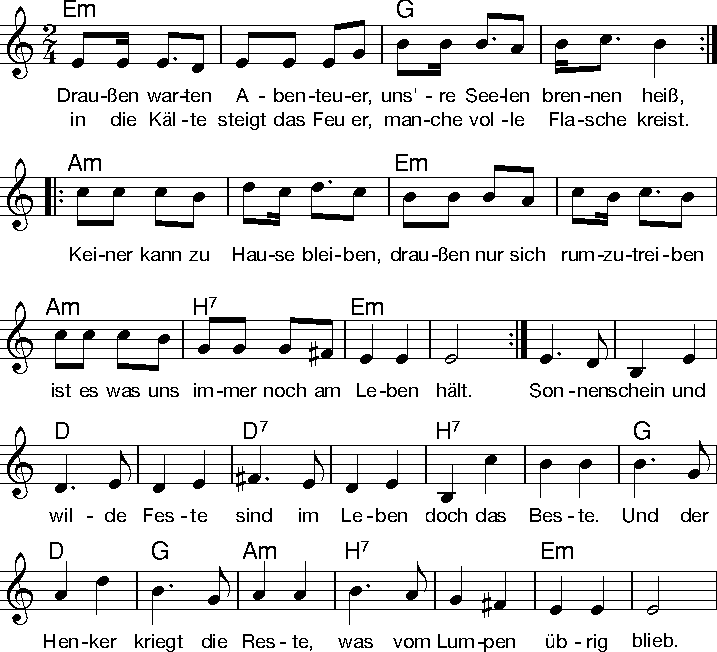
\includegraphics[draft=false, width=1\textwidth]{Noten/Lied081.pdf}

\beginverse
\[Em]Morgens brummt so mancher Schädel, \[G]aber das geht auch vorbei,
zu \[Em]Hause wartet manches Mädel, \[G]meinet noch, wir wären treu.
\lrep \[Am]Wer wollt uns was übel nehmen, \[Em]wofür sollten wir uns schämen?
\[Am]Nur hier draußen \[H7]auf der Straße \[Em]sind wir frei. \rrep
\endverse

\beginchorus
\[Em]Sonnenschein und \[D]wilde Feste 
\[D7]sind im Leben \[H7]doch das Beste
\[G]und der \[D]Henker \[G]kriegt die \[Am]Reste, 
\[H7]was vom Lumpen \[Em]übrig blieb.
\endchorus

\beginverse
^Lumpen, Lampen, Pferdewagen, ^Pfeifendunst, Gesang und Wein,
^Soweit uns die Füße tragen, ^fahren wir jahraus, jahrein.
\lrep ^Fremde Länder zu gewinnen, ^neues Leben zu beginnen,
^was auf dieser ^Erde kann denn ^schöner sein? \rrep
\endverse

\beginchorus
\lrep \[Em]Sonnenschein und \[D]wilde Feste
\[D7]sind im Leben \[H7]doch das Beste
\[G]und der \[D]Henker \[G]kriegt die \[Am]Reste,
\[H7]was vom Lumpen \[Em]übrig blieb.\rrep
\endchorus

\endsong
